To evaluate the impact of the system's learning capabilities, the perceived quality of recommendations was compared between the initial cold-start conversation (Use Case 2) and the conversation after the agent was retrained with the user's feedback (Use Case 3). The average scores for each metric are visualized in Figure~\ref{FIG:REC_METRICS} and presented in Table~\ref{TAB:REC_RESULTS}.

\begin{figure}[Recommendation Metrics]{FIG:REC_METRICS}{Comparison of recommendation evaluation results.}
    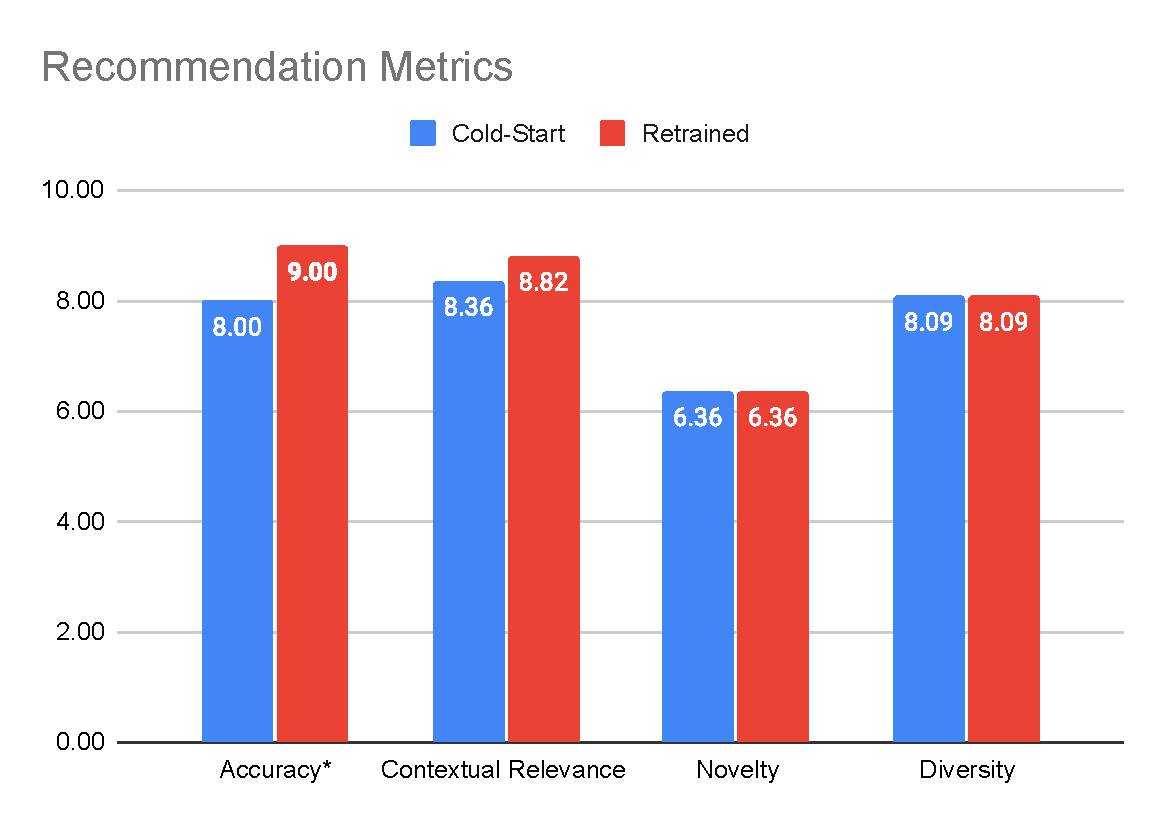
\includegraphics[width=0.8\textwidth]{rec_metrics.pdf}
\end{figure}

\begin{table}[Recommendation Quality Scores]{TAB:REC_RESULTS}{Average scores for recommendation quality (1-10 scale).}
    \begin{tabular}{l c c}
        \hline
        \textbf{Metric} & \textbf{Cold-Start (UC2)} & \textbf{Retrained (UC3)} \\
        \hline
        Accuracy* & 8.00 & 9.00 \\
        Contextual Relevance & 8.36 & 8.82 \\
        Novelty & 6.36 & 6.36 \\
        Diversity & 8.09 & 8.09 \\
        \hline
        \multicolumn{3}{l}{\footnotesize{*Indicates a statistically significant improvement ($p < 0.05$)}}
    \end{tabular}
\end{table}

A one-tailed, paired-samples t-test was conducted to assess the statistical significance of these changes. The results show a \textbf{statistically significant improvement in perceived Accuracy} after retraining (p = 0.042), indicating that users found the recommendations to be more relevant after the agent had learned from their initial feedback. While there was also a slight increase in Contextual Relevance, this change, along with Novelty and Diversity, was not found to be statistically significant.